% Send to Mandar,Jayesh,Arnab,Deepak and perhaps Rahee
\documentclass{article}
\newcommand{\beq}{\begin{equation}}
\newcommand{\eeq}{\end{equation}}
\newcommand{\ber}{\begin{eqnarray}}
\newcommand{\eer}{\end{eqnarray}}
\newcommand{\nn}{\nonumber}
\newcommand{\dd}[2]{\frac{d}{d{#2}}{(#1)} }
\newcommand{\pdd}[2]{\frac{\partial}{\partial{#2}}{(#1)} }
\usepackage{amsmath}
\usepackage{amsfonts}
\usepackage{url}
\usepackage{graphicx}
\usepackage{caption}
\usepackage{subcaption}
\usepackage{multirow}
\begin{document}
\title{Circle identification using Convolutional Neural Networks in TensorFlow}
\author{Nachiket Gokhale\footnote{Conversations with Arnab Majumdar and Mandar Kulkarni are acknowledged and much appreciated.}}
\date{\today}
\maketitle
\section{Introduction}
We consider a dataset consisting of images of stiffness of the type shown in Figure (\ref{fig:sampleimages}). All images are 32 pixels (x direction) by 128 pixels (y-direction). Unlike standard RGB images which have three channels, these images have only one channel. So, the shape of each image is $(32,128,1)$. The value of the background stiffness is $1$ and the value of the circle stiffness is a real number which ranges from $2.0$ to $5.0$. Each image contains only one circle or is homogeneous (no circles). We consider the following problems
\begin{enumerate}
\item{\textbf{Binary classification}: Given a stiffness image classify it into homogneous (label 0)or having an inclusion (label 1).}
\item{\textbf{Predicting stiffness location:} Given a stiffness image containing a circle find the center of the circle.}
\item{\textbf{Predicting stiffness value:} Given a stiffness image containing a circle find the value of the stiffness of the circle.}
\item{\textbf{Predicting circle radius:} Given a stiffness image containing a circle find the radius of the circle.}
\end{enumerate}
\begin{figure}
  \centering
  \begin{subfigure}[b]{0.45\textwidth}
    \centering
    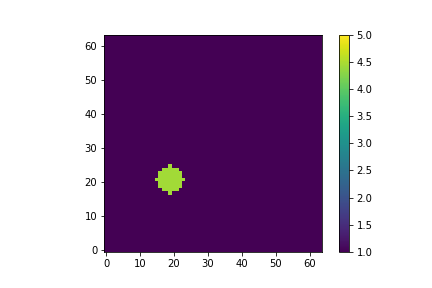
\includegraphics[totalheight=4cm]{circle_id/sample0.png}
    \caption{Sample image 1}
  \end{subfigure}
  %
  \begin{subfigure}[b]{0.45\textwidth}
    \centering
    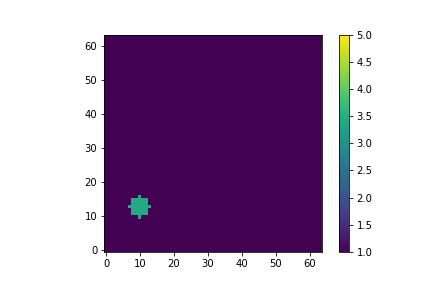
\includegraphics[totalheight=4cm]{circle_id/sample1.png}
    \caption{Sample image 2}
  \end{subfigure}
  %
  \begin{subfigure}[b]{0.45\textwidth}
    \centering
    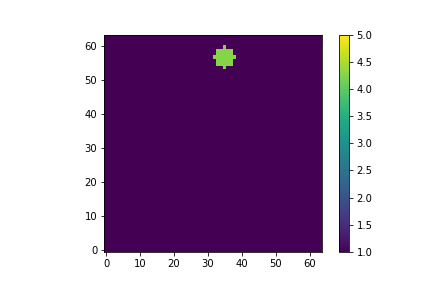
\includegraphics[totalheight=4cm]{circle_id/sample2.png}
    \caption{Sample image 3}
  \end{subfigure}
  \begin{subfigure}[b]{0.45\textwidth}
    \centering
    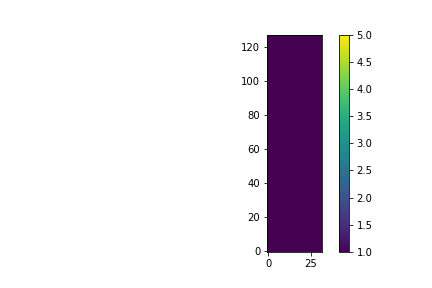
\includegraphics[totalheight=4cm]{circle_id/sample3.png}
    \caption{Sample image 4 (no circle)}
  \end{subfigure}
  %
  \begin{subfigure}[b]{0.45\textwidth}
    \centering
    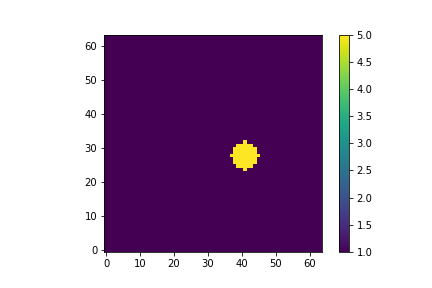
\includegraphics[totalheight=4cm]{circle_id/sample4.png}
    \caption{Sample image 5}
  \end{subfigure}
  %
  \begin{subfigure}[b]{0.45\textwidth}
    \centering
    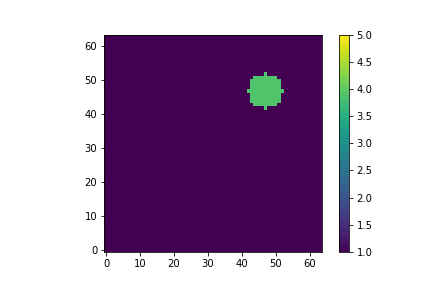
\includegraphics[totalheight=4cm]{circle_id/sample5.png}
    \caption{Sample image 6}
  \end{subfigure}
\caption{\label{fig:sampleimages} Sample images in the image dataset.}
\end{figure}
%
\section{Preliminaries}
We first define two parameters '\textbf{min\_delta}' and '\textbf{patience}'. From the TensorFlow manual '\textbf{min\_delta}'is the ``minimum change in the monitored quantity to qualify as an improvement, i.e. an absolute change of less than min\_delta, will count as no improvement''. In our case, the monitored quantity is the validation loss. '\textbf{patience}' is the ``number of epochs with no improvement after which training will be stopped''.
\section{Binary classification}
 The parameters used for 'Binary classification' are given in Table (\ref{tab:binaryparam}).We first feature scale the images using their standard deviation and mean using the 'StandardScaler' in 'scikit-learn'. The architecture of the CNN\footnote{This architecture is taken 'as is' from a CNN to classify images into two categories: 'cat' or 'dog'} is shown in Figure (\ref{fig:binary_model}). Both the convolutional layers have $32$ filters with a kernel size of $3$. The max-pooling layers have a pool size of $2$ and a stride of $2$. The activation for the output layer is 'sigmoid' and the threshold probability for positive images is $0.5$. The good results that are seen are a consequence of the large number of training parameters. It is also observed that the training of the CNN is quite strongly dependent on the initial random choice of parameters. The metrics for binary classification are shown in Figure (\ref{fig:binarymetrics}). We get an accuracy score of $1.0$ right from the start. The confusion matrix is shown in Table (\ref{tab:confusionbinary}). 
\begin{table}
  \centering
  \begin{tabular}{|c|c|}
    \hline
    Parameter & Value \\
    \hline
    Number of training examples   & 1024 \\
    Number of validation examples & 205 \\
    Number of test examples       & 1024 \\
    Maximum number of epochs      & 512 \\
    min{\_}delta      & 10$^{-4}$\\
    patience                      & 10  \\
    Trainable parameters          & 747105\\
    Optimizer         & 'adam'     \\
    Loss function     & 'binary\_crossentropy' \\
    Number of positive training examples (with circle) & 721\\
    Number of negative training examples (without circle) & 303\\
    \hline
  \end{tabular}
  \caption{\label{tab:binaryparam} Parameters for binary classification}
\end{table}
\begin{figure}
   \centering
    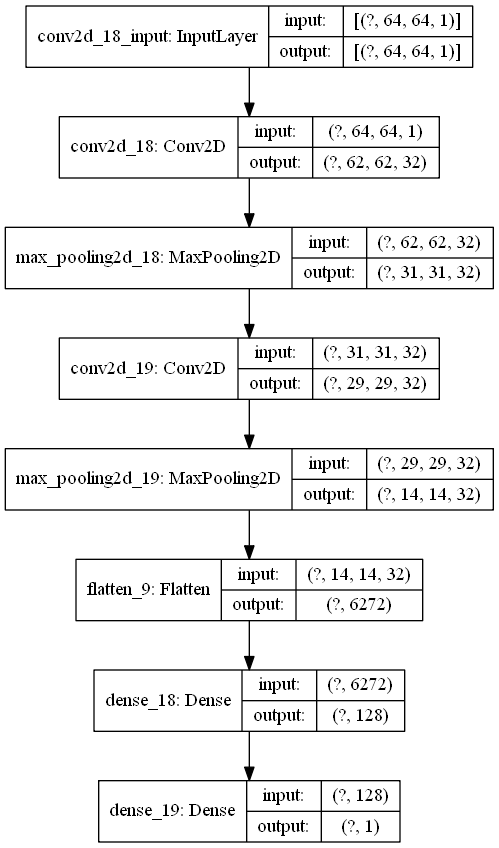
\includegraphics[totalheight=16cm]{circle_id/binary/model.png}
  \caption{\label{fig:binary_model} CNN for binary classification.}
\end{figure}
%
\begin{figure}
\centering
\begin{subfigure}[b]{0.45\textwidth}
    \centering
    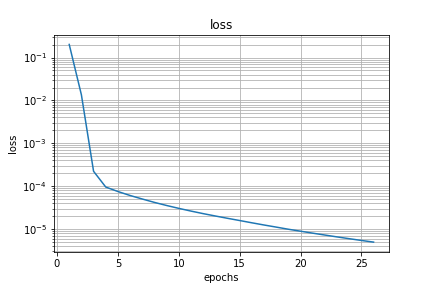
\includegraphics[totalheight=4cm]{circle_id/binary/plotloss.png}
    \caption{Training loss}
  \end{subfigure}
%
\begin{subfigure}[b]{0.45\textwidth}
    \centering
    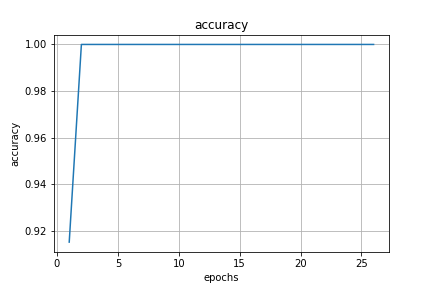
\includegraphics[totalheight=4cm]{circle_id/binary/plotaccuracy.png}
    \caption{Training accuracy}
  \end{subfigure}
%
\begin{subfigure}[b]{0.45\textwidth}
    \centering
    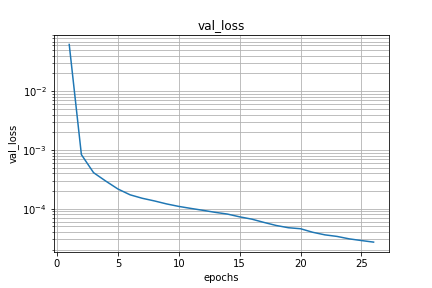
\includegraphics[totalheight=4cm]{circle_id/binary/plotval_loss.png}
    \caption{Validation loss}
  \end{subfigure}
%
\begin{subfigure}[b]{0.45\textwidth}
    \centering
    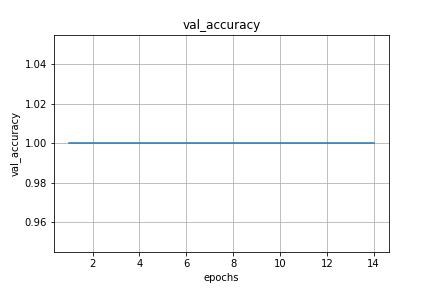
\includegraphics[totalheight=4cm]{circle_id/binary/plotval_accuracy.png}
    \caption{Validation accuracy}
  \end{subfigure}
\caption{\label{fig:binarymetrics} Metrics for binary classification.}
\end{figure}
%
\begin{table}
\begin{center}
  \begin{tabular}{cccc}
    \cline{3-4}
    & & \multicolumn{2}{|c|}{Actual class}  \\
    \cline{3-4}
    & & \multicolumn{1}{|c|}{Circle} &  \multicolumn{1}{|c|}{No Circle}\\
    \hline
    \multicolumn{1}{|c}{Predicted} & \multicolumn{1}{|c|}{Circle} & \multicolumn{1}{|c|}{307} & \multicolumn{1}{|c|}{0} \\
    \cline{2-4}
    \multicolumn{1}{|c}{class} & \multicolumn{1}{|c|}{no circle} & \multicolumn{1}{|c|}{1} & \multicolumn{1}{|c|}{716}\\
    \hline
  \end{tabular}
\end{center}
\caption{\label{tab:confusionbinary} Confusion matrix for binary classification.}
\end{table}
%
\section{Predicting stiffness location}
%
The parameters used for 'Stiffness location' are given in Table (\ref{tab:stifflocparam}). We first feature scale the images using their standard deviation and mean using the 'StandardScaler' in 'scikit-learn'. We also feature scale the predicted values, because of the range of scales involved. The CNN architecture is the same as the one used in 'Binary classification' shown in Figure (\ref{fig:binary_model}) with the following differences:
\begin{enumerate}
\item{We have two output units instead of one.}
\item{There is no activation for the output layer.}
\end{enumerate}
The training loss and validation loss are shown in Figure (\ref{fig:locationmetrics}) and the errors in location are shown in Figure (\ref{fig:locationerror}).
\begin{table}
  \centering
  \begin{tabular}{|c|c|}
    \hline
    Parameter & Value \\
    \hline
    Number of training examples   & 1024 \\
    Number of validation examples & 205 \\
    Number of training examples   & 1024 \\
    Maximum number of epochs      & 512 \\
    min{\_}delta      & 10$^{-4}$\\
    patience                      & 10  \\
    Trainable parameters          & 812770\\
    Optimizer         & 'adam'     \\
    Loss function     & 'mse' (mean squared error) \\
    \hline
  \end{tabular}
  \caption{\label{tab:stifflocparam} Parameters for stiffness location}
\end{table}
%
\begin{figure}
\centering
\begin{subfigure}[b]{0.45\textwidth}
    \centering
    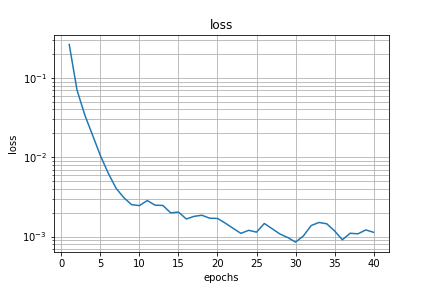
\includegraphics[totalheight=4cm]{circle_id/location/plotloss.png}
    \caption{Training loss}
  \end{subfigure}
%
\begin{subfigure}[b]{0.45\textwidth}
    \centering
    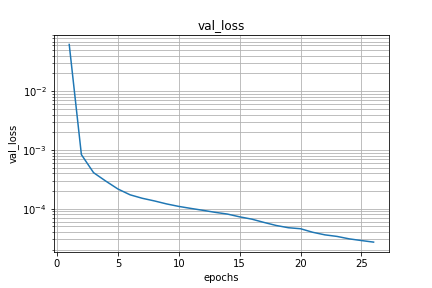
\includegraphics[totalheight=4cm]{circle_id/binary/plotval_loss.png}
    \caption{Validation loss}
  \end{subfigure}
%
\caption{\label{fig:locationmetrics} Metrics for stiffness location identification.}
\end{figure}
%
\begin{figure}
\centering
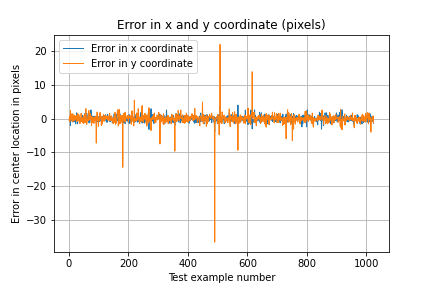
\includegraphics{circle_id/location/plotabserror.png}
\caption{\label{fig:locationerror} Error in pixels for stiffness location identification.}
\end{figure}

\section{Predicting stiffness value}
%
\section{Predicting circle radius}
%
\end{document}
